\documentclass{article}

\usepackage{times}
\usepackage{fancyhdr}
\usepackage{listings}
\usepackage{xcolor}
\usepackage{textcomp}
\usepackage{graphicx}
\usepackage{float}
\usepackage{amsmath}
\usepackage{pbox}

\lstdefinestyle{customc++}{
  belowcaptionskip=1\baselineskip,
  breaklines=true,
  frame=L,
  xleftmargin=\parindent,
  language=C,
  showstringspaces=false,
  basicstyle=\footnotesize\ttfamily,
  keywordstyle=\bfseries\color{green!40!black},
  commentstyle=\itshape\color{purple!40!black},
  identifierstyle=\color{blue},
  stringstyle=\color{orange},
}

\lstset{escapechar=@,style=customc++,captionpos=b}

\begin{document}

% Article top matter
\title{Implementation of Particle Swarm Optimization for the multi-dimensional knapsack problem \\
\vspace{2 mm} {\large Coursework Artificial Intelligence 2}}
\author{JeGa\\
        Applied Computer Science\\
		HTWG Konstanz}
\date{\today}
\maketitle

\begin{abstract}
Particle Swarm Optimization (PSO) is a metaheuristic search algorithm which uses a swarm of solutions/particles to iteratively optimize a problem. PSO was intentionally designed by Kennedy and Eberhart \cite{bib-continues} for continues optimization problems. Later, several papers were published that cover PSO for discrete search spaces. This document describes the implementation of the discrete binary PSO algorithm to solve the multi-dimensional knapsack problem.
\end{abstract}

\newpage
\cfoot[\thepage]{}

\tableofcontents

\newpage

\section{Introduction}
\label{lbl-intro}
Because PSO was designed for continues problems, some changes need to be done to use it for discrete problems. This document covers shortly the PSO for continues problems (\ref{lbl-pso-cont}) and the changes to be made to use PSO for discrete problems (\ref{lbl-pso-disc}). The next chapter (\ref{lbl-mknap}) describes the multidimensional knapsack problem and the adaption of the PSO.
Implementation details are outlined in chapter \ref{lbl-impl}. After that the performance of the algorithm and implementation is analysed (\ref{lbl-tests}). The application and the improvements that can be made are described in chapter \ref{lbl-app} and \ref{lbl-impr}. At last, a paper which presents improvements for the discrete binary PSO is reviewed (\ref{lbl-rev}).

\section{PSO for continues problems}
\label{lbl-pso-cont}
Particle Swarm Optimization is a swarm algorithm based on the flocking behaviour of birds where a swarm of birds searches for food. Every bird (particle) uses its own knowledge (cognitive part) and the swarms knowledge (social part) to direct its search towards the food. In PSO, a particle represents a possible solution. It consist of a position $x_i$ and a velocity $v_i$. Each particle saves its best position (particle best - pBest). Additionally the best position of all particles in the swarm is saved (global best - gbest). Each particle updates its position based on the current velocity, the particles best position and the global best position. If the problem is multidimensional, based on each dimension $d$ of the solution vector, the new velocity/position must be calculated.
\begin{equation}
\label{formula-1}
v_i = \omega * v_i + c_1 * rand_1 * (x_{pbest} - x_i) + c_2 * rand_2 * (x_{gbest} - x_i)
\end{equation}
\begin{equation}
\label{formula-2}
x_i = x_i + v_i
\end{equation}

$\omega$ is the inertia weight which specify how strong the current velocity contributes to the new velocity. $c_1$ and $c_2$ are constants which weight the personal and the swarms evidence. $rand_1$ and $rand_2$ are random values from $[0,1]$. Additionally, the new velocity $v_i$ is limited by a constant $v_{max}$.

\section{PSO for discrete binary problems}
\label{lbl-pso-disc}
To use PSO for discrete binary problems, some changes need to be made. Unlike in continues space, a multidimensional solution vector (position) consist now of discrete binary values (0/1). The velocity of a particle is expressed as a vector of probabilities, that the elements at each dimension have the value 1 (rate of change). This means, a particle flies fast if all the binary values change and slow if nothing changes. However, the velocity formula remains the same, but the calculation of the new position changes slightly. At first, to limit the velocity value to a valid probability, a logistic transformation with the sigmoid function is made.
\begin{equation}
\label{formula-3}
S(v_i) = 1.0 / (1.0 + e^{(-v_i)})
\end{equation}

The output of formula is a velocity limited with the sigmoid function to $[0.0, 1.0]$. To calculate the new position, an update strategy is needed. The used update strategy is the original strategy from Kennedy and Eberhart \cite{bib-discrete}.

\begin{equation}
p_i = \left\{ 
\begin{array}{l l}
  1 & \quad \text{$rand() < S(v_i)$}\\
  0 & \quad \text{otherwise}
\end{array} \right.
\end{equation}


\section{Multidimensional knapsack problem}
\label{lbl-mknap}
Because the multidimensional (multi-constraint) knapsack problem is already described in detail in a lot of papers, it is only briefly described here. To sum up, a number of elements need to be packed into a knapsack. Each element has a profit value, and several constraint values. The aim is, to maximize the profit (fitness value) while not violating any constraint. A solution is described as a binary vector with the dimension as the number of elements to pack. 1 means the element is in the knapsack, 0 means it is not in the knapsack. \\ An important addition to the traditional discrete PSO are the constraint values. Special care has to be taken to identify invalid solutions.\\

A particle consists of the following information (figure \ref{fig-particle}):
\begin{itemize}
\item Binary solution vector (the current position)
\item Real velocity vector
\item pBest value and position
\end{itemize}

\begin{figure}[H]
    \centering
    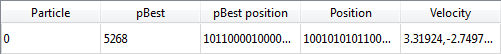
\includegraphics[width=250px]{images/particle.PNG}
    \caption{Particle}
    \label{fig-particle}
\end{figure}

\section{Implementation}
\label{lbl-impl}
This chapter describes the implementation in detail and shows some extracts from the source code. Figure \ref{fig-algo} shows the flow diagram of the implemented algorithm. The single steps and their implementation are outlined in the following sections.

\begin{figure}[H]
    \centering
    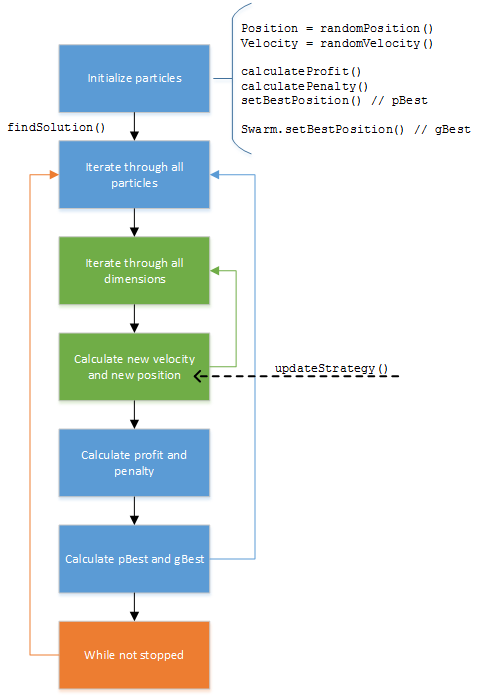
\includegraphics[width=180px]{images/algo.png}
    \caption{Algorithm}
    \label{fig-algo}
\end{figure}

\subsection{Algorithm}
At first, the particles are initialized with random positions and random velocities. After that, the profit of the particular solution is calculated. If the position is invalid and violates a constrained, the penalty value is calculated and subtracted from the fitness value. The fitness value is saved as pBest value. The highest profit of all particles is saved as the swarms gBest value. It is very likely, that the particles have invalid positions, so at this point the penalty values are very high.

\begin{lstlisting}[caption="Solver.cpp"]
for (auto &i : swarm.getParticles()) {
	Solution position = getRandomSolution();
   	Velocity velocity = getRandomVelocity();

	i.setPosition(position);
	i.setVelocity(velocity);
	
	// Fitness value / Profit of the solution/position.
	int profit = calculateProfit(position);
	profit -= calculatePenalty(position, profit);
	
	// ... Set gBest and pBest
}
\end{lstlisting}

After initialization, the method \lstinline$findSolution()$ is called, to iterate through all particles of the swarm. For each dimension of the particles the formula \ref{formula-1} and \ref{formula-2} are applied. Dependent on \lstinline{(pBestD - currentPositionD)} and \lstinline{(gBestD - currentPositionD)} the output values are \lstinline$0$, \lstinline$-1$ or \lstinline$1$ and change the probability of the position to be 1 or 0.

\begin{lstlisting}[caption="Solver.cpp"]
double newVelocityD = parameters.getInertiaWeight() *
	currentVelocityD +
	parameters.getConstant1() * randomParticleNumber *
	(pBestD - currentPositionD) +
	parameters.getConstant2() * randomGlobalNumber *
	(gBestD - currentPositionD);

if (newVelocityD > parameters.getVMax())
    newVelocityD = parameters.getVMax();
else if (newVelocityD < -parameters.getVMax())
    newVelocityD = -parameters.getVMax();

int newPositionD = updateStrategy->updatePosition(
	currentPositionD, newVelocityD);
\end{lstlisting}

At last, the profit and the penalty values are calculated. With this information the pBest and gBest values can be updated. If the particles current fitness value is higher than its pBest value, the current value is the new pBest. If this is true, this value could be better than the swarms gBest value. So gBest is updated if pBest is higher.

\begin{lstlisting}[caption="Solver.cpp"]
int pBestTmp = calculateProfit(i.getPosition());
pBestTmp -= calculatePenalty(i.getPosition(), pBestTmp);

// Update pBest and gBest position/solution
if (pBestTmp > i.getBestValue()) {
	i.setBestPositionAndValue(i.getPosition(), pBestTmp);
	if (pBestTmp > swarm.getBestValue()) {
	    swarm.setBestPositionAndValue(
	    	i.getPosition(), pBestTmp);
	}
}
\end{lstlisting}

\subsection{Update strategies}
There are several strategies available, to update the particles position based on the velocity. The current used strategy in the implementation is the original strategy from Kennedy and Eberhart \cite{bib-discrete}.The improved update strategy from Qi Shen is also implemented. The implementation of the standard update strategy is showed in the following code extract.

\begin{lstlisting}[caption="UpdateStrategy.cpp"]
// Logistic transformation
velocity = 1.0 / (1.0 + exp(-velocity));

double randomValue = getRandomDoubleValue(0.0, 1.0);

int newPositionD;
if (randomValue < velocity)
    newPositionD = 1;
else
    newPositionD = 0;
\end{lstlisting}

The variable \lstinline{velocity} is the output of the logistic transformation. If the velocity is high, the probability of the position in the current dimension that it gets the value 1 is high. The probability that the value is 0 is low.

\subsection{Penalty function}
A very important part of the algorithm is the penalty function. Because the knapsack problem has multiple constraints, invalid positions can occur. The penalty function therefore adjusts the fitness value to a valid fitness value (based on several different parameters). There are a many penalty functions to choose from. It is important, to choose a good penalty function, because it does strongly influence the optimization capabilities of PSO. If the penalty function is too weak, invalid positions are more likely and the algorithm does not perform well. If it is too large, it negatively influences the performance of PSO.\\ \\
In this implementation, a penalty function from Oken \cite{bib-penalty} is used. It uses the current fitness value of a particles position to weight the penalty. If a solution has a very large profit and is invalid, it gets a high penalty.

\begin{lstlisting}[caption="Solver.cpp"]
// Check constraint i
int dist = checkConstraint(newPosition, i);

if (dist) {
	// Constraint violated
	
	// ...
	
	// Penalty function
	int penalty = (int) (pBestTmp *
		(((double) dist) / (double) diff));
		
	// Sum up with penalty function
	penaltyValue += penalty;
}
\end{lstlisting}

\lstinline{dist} is the difference between the constraints maximal capacity and the current (invalid) capacity. \lstinline{diff} is the minimum of the violated constraints maximal capacity and all other constraints capacity minus the current violated constraints capacity.

\subsection{Parameter}
The available parameters are explained in the following table.\\

\begin{tabular}{|l|l|}
	\hline
	Inertia weight ($\omega$) & \pbox{10cm}{Specifies the impact of the current velocity to the new velocity. If the inertia weight is too high, the particles do not change their positions (they have no confidence in the other particles knowledge). Also a low $V_{max}$ could balance this, the behaviour is not very good. A too low inertia weight results in a too heavy change of the particles position. Figure \ref{fig-inertia} shows the differences between low and high inertia values.} \\ \hline
	Maximal velocity ($V_{max}$) & \pbox{10cm}{Limits the velocity. A lesser $V_{max}$ value allows more differences in the particles position. However, it does take longer time until they converge. If the $V_{max}$ value is 2, the output velocities of the sigmoid function can only be in the range of [0.12, 0.88]. So if the velocity is very high (e.g. v = 10.0, Sig(v) = 0.88), the possibility that the particles position is 0 (1 - 0.88) is still there. If $V_{max}$ is too high, particles can fly past good positions. If it is too small, it could be that good positions are never visited. Figure \ref{fig-vmax} shows the difference between a low and high $V_{max}$ value.} \\ \hline
	Constant 1 ($c_1$) & Weights the evidence of the particle \\ \hline
	Constant 2 ($c_2$) & Weights the evidence of the swarm \\ \hline
	Particle count & \pbox{10cm}{Number of particles in the swarm. With many particles the probability of searching different areas raises. However, with each particle the computational effort raises strongly too. Tests showed that a swarm size of 20 particles were totally enough to search a great area.} \\ \hline
\end{tabular}\\

\begin{figure}[H]
    \centering
    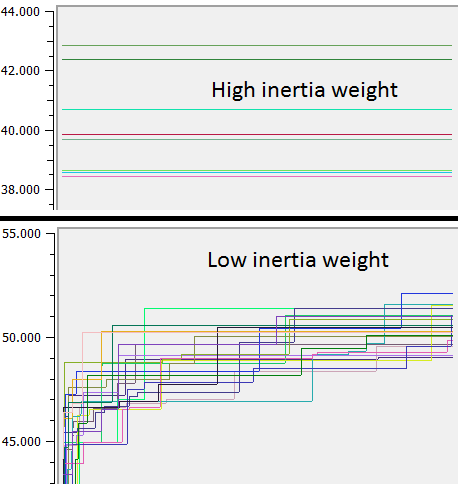
\includegraphics[width=200px]{images/inertia.PNG}
    \caption{Inertia weight}
    \label{fig-inertia}
\end{figure}

\begin{figure}[H]
    \centering
    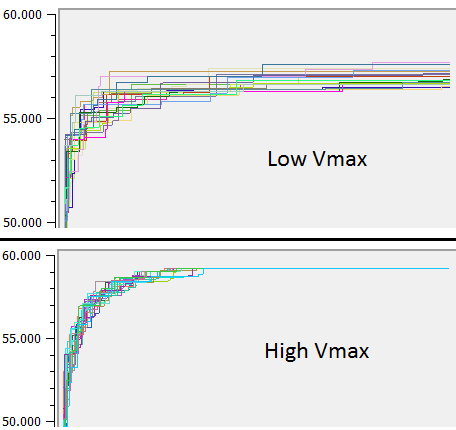
\includegraphics[width=200px]{images/vmax.PNG}
    \caption{Vmax}
    \label{fig-vmax}
\end{figure}

\section{Tests}
\label{lbl-tests}
For the tests, the \lstinline$mknapcb1.txt$ problems from the OR library were used.  Dependent on the problem, it can be, that the start values are very low ($< 0$). The very low start values are a result of the penalty function. Because all particles are initialized with random values, it is very likely that the particles violate a constraint and are invalid. Because of that, the particles get a very high penalty.\\

The following table shows tests with different parameters. The first problem from \lstinline$mknapcb1.txt$ is used to do the tests. The values are averaged over 30 iterations. The parameter column has the following meaning: (Number of particles, iterations, $\omega$, $c_1$, $c_2$, $V_{max}$). \\

\begin{tabular}{|l|l|l|l|l|l|}
	\hline
	Optimum & Parameter & Best & Worst & Mean Optimum & Mean Time (ms) \\ \hline
	24381 & (5 500 1 2 2 6) & 22980 & 19880 & 21310.5 & 271.233 \\ \hline
	24381 & (10 500 1 2 2 6) & 22910 & 20463 & 22017 & 546.533 \\ \hline
	24381 & (15 500 1 2 2 6) & 23339 & 21801 & 22552.7 & 824.967 \\ \hline
	24381 & (20 500 1 2 2 6) & 23414 & 21681 & 22684.3 & 1101.57 \\ \hline
	24381 & (25 500 1 2 2 6) & 23432 & 21740 & 22777.1 & 1361.77 \\ \hline
	24381 & (30 500 1 2 2 6) & 23890 & 21795 & 22998.5 & 1621.9 \\ \hline
	24381 & (20 500 0.1 2 2 6) & 18388 & 5270 & 12398.8 & 1114.17 \\ \hline
	24381 & (20 500 0.5 2 2 6) & 19583 & 16561 & 18434.2 & 1121.3 \\ \hline
	24381 & (20 500 0.8 2 2 6) & 21322 & 19616 & 20363.1 & 1127.33 \\ \hline
	24381 & (20 500 0.9 2 2 6) & 22628 & 20890 & 21536.7 & 1106.03 \\ \hline
	24381 & (20 500 1 2 2 6) & 23605 & 21656 & 22717.4 & 1088 \\ \hline
	24381 & (20 500 1.1 2 2 6) & 22600 & 19790 & 21510.5 & 1079.07 \\ \hline
	24381 & (20 500 1.2 2 2 6) & 22703 & 19756 & 21217.7 & 1084.03 \\ \hline
	24381 & (20 500 1.5 2 2 6) & 19286 & -28318 & 4117.73 & 1123.63 \\ \hline
	24381 & (20 500 1 0.1 1 6) & 23584 & 21820 & 22755.8 & 1089.07 \\ \hline
	24381 & (20 500 1 0.5 1 6) & 23594 & 21876 & 22924.1 & 1082.73 \\ \hline
	24381 & (20 500 1 1 1 6) & 23730 & 21823 & 22965.2 & 1083.57 \\ \hline
	24381 & (20 500 1 2 1 6) & 23863 & 22848 & 23365.6 & 1080.5 \\ \hline
	24381 & (20 500 1 3 1 6) & 24081 & 23129 & 23545.4 & 1085.2 \\ \hline
	24381 & (20 500 1 5 1 6) & 24133 & 22981 & 23599 & 1088.27 \\ \hline
	24381 & (20 500 1 10 1 6) & 24229 & 23079 & 23602.5 & 1088.3 \\ \hline
	24381 & (20 500 1 1 0.1 6) & 23661 & 22185 & 22937.3 & 1090 \\ \hline
	24381 & (20 500 1 1 1 6) & 23652 & 21661 & 23062.7 & 1084.83 \\ \hline
	24381 & (20 500 1 1 5 6) & 22889 & 20498 & 22035 & 1075.4 \\ \hline
	24381 & (20 500 1 2 2 0.1) & 13937 & -8554 & 1908.87 & 1107.83 \\ \hline
	24381 & (20 500 1 2 2 0.5) & 19180 & 7509 & 13612.7 & 1121.43 \\ \hline
	24381 & (20 500 1 2 2 1) & 21082 & 18077 & 19005.4 & 1117.33 \\ \hline
	24381 & (20 500 1 2 2 2) & 22442 & 20789 & 21531.6 & 1103.97 \\ \hline
	24381 & (20 500 1 2 2 3) & 24052 & 22373 & 23139.8 & 1097.33 \\ \hline
	24381 & (20 500 1 2 2 4) & 23885 & 22345 & 23447.7 & 1087.47 \\ \hline
	24381 & (20 500 1 2 2 5) & 23844 & 22051 & 23026.8 & 1071.5 \\ \hline
	24381 & (20 500 1 2 2 10) & 23102 & 21839 & 22503.6 & 1074.47 \\ \hline
	24381 & (20 500 1 2 2 20) & 23276 & 21441 & 22647.6 & 1079.47 \\ \hline
\end{tabular} \\\\

The tests show that a parameter setting with a high $c_1$ value result in good optimization capabilities (fitness value 24229, optimal fitness value 24381). The best found configuration is displayed in figure \ref{fig-param}.

\begin{figure}[H]
    \centering
    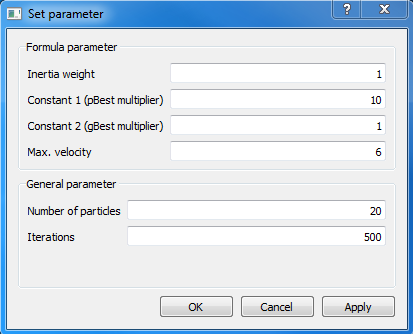
\includegraphics[width=200px]{images/parameter.PNG}
    \caption{Parameter}
    \label{fig-param}
\end{figure}

The implemented PSO does converge towards 5\% below the optimum. it does not work optimal, so there are some improvements to do, which are outlined in chapter \ref{lbl-impr}. However, one can see that PSO converges very fast. There are only a few steps needed, until all particles converge to a common optimum. Figure \ref{fig-p30_200it_p1} shows the gBest value of the swarm with a iteration value of 200. Figure \ref{fig-p30_200it_p1_particles} shows the particles and how they converge to a common optimum.

\begin{figure}[H]
    \centering
    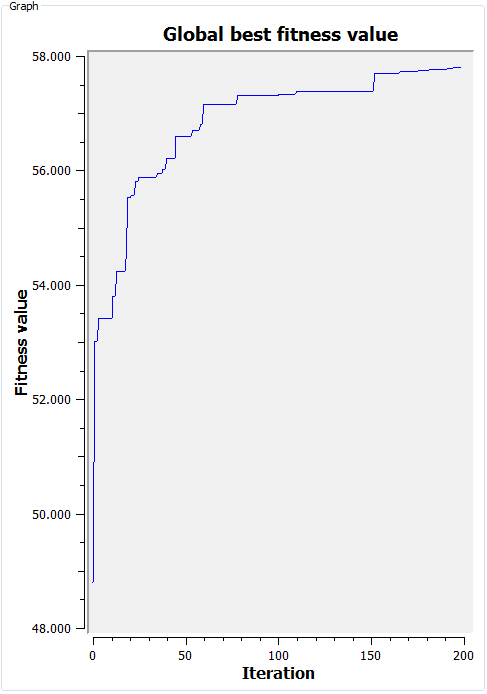
\includegraphics[width=160px]{images/p30_200it_p1.PNG}
    \caption{Global swarm optimum}
    \label{fig-p30_200it_p1}
\end{figure}

\begin{figure}[H]
    \centering
    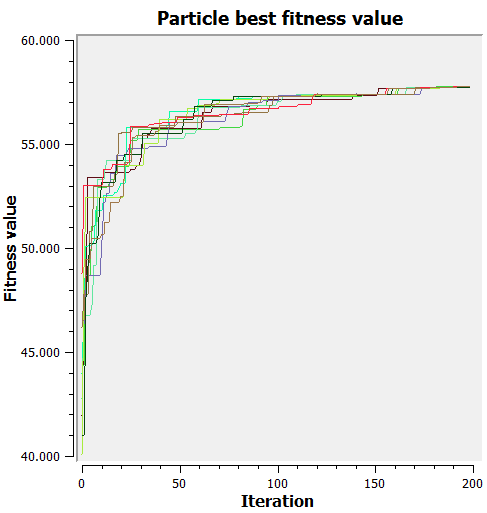
\includegraphics[width=200px]{images/p30_200it_p1_particles.PNG}
    \caption{Particles optimum}
    \label{fig-p30_200it_p1_particles}
\end{figure}

In figure \ref{fig-particles_optimum} one can see, that all particles have almost the same pBest value.

\begin{figure}[H]
    \centering
    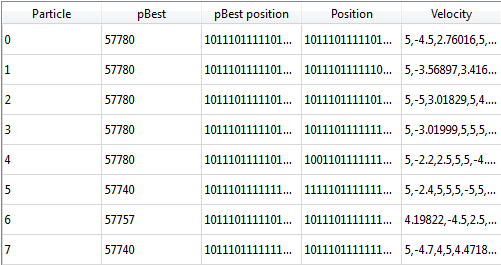
\includegraphics[width=250px]{images/particles_optimum.PNG}
    \caption{Particles optimum}
    \label{fig-particles_optimum}
\end{figure}

\section{Application}
\label{lbl-app}
The application is able to parse files from the OR library with the same format as $mknapcb1.txt$. The GUI   provides tables to view the problems and its values. The user is able to set different parameters via the File-settings dialogue. He can choose between automatic or manual (step by step) iteration. Note that the GUI is made only for testing purpose, so there are still some improvements to do. The algorithm is done in the GUI thread, so the GUI blocks (algorithm needs a worker thread). To run the algorithm, a problem file has to be parsed. After that, a problem can selected from the table. With the button "Solve Problem" the algorithm is started. The parameters can be set with "File-set parameter".

\begin{figure}[H]
    \centering
    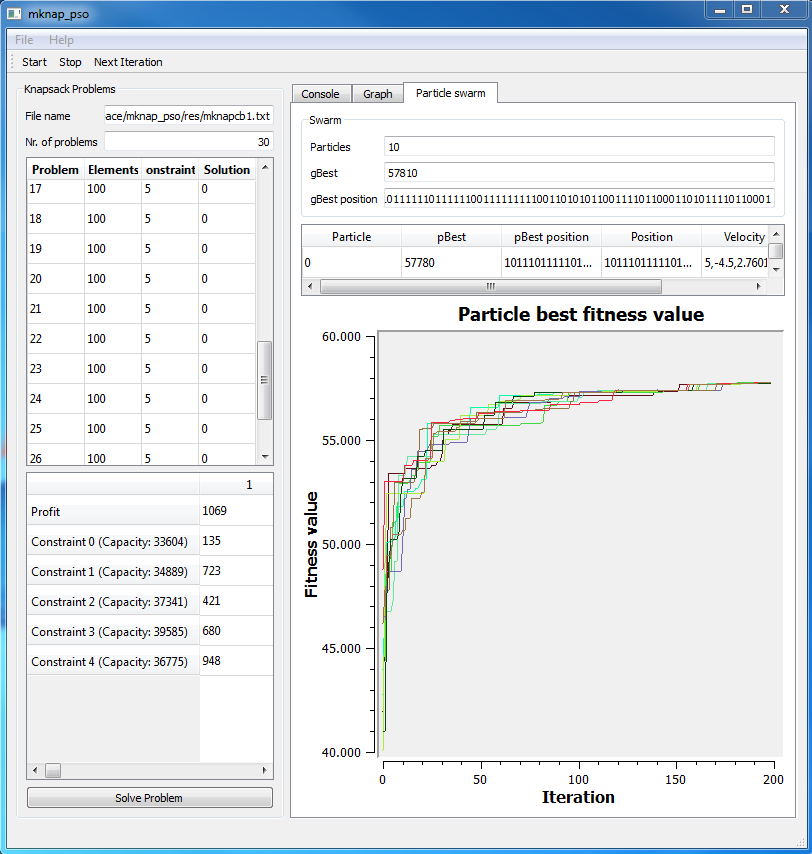
\includegraphics[width=220px]{images/image_main.PNG}
    \caption{Application}
    \label{fig-app}
\end{figure}

\section{Critique and improvements}
\label{lbl-impr}
The discrete PSO does converge towards the optimum, however it does not work optimal. The global best position remains dependent of the problem in average of about 5\% below the optimal value. One problem is the penalty function which could be optimized. It is difficult, to find a suitable penalty function for constrained values. A different approach would be to use a repair mechanism to turn invalid solutions to valid solutions. Another optimization is to use a local best position instead of the swarms best position for the calculation of the velocity. In this case, only the $n$ nearest neighbour particles are used to calculate the lBest value. To further improve the algorithm, the inertia weight could be variable which changes over the iteration time (no constant). A linear change from 0.9 to 0.4 for the inertia weight would help, to search at the beginning in more global areas. With more iterations PSO searches more in local areas. A advantage of PSO is, that there are only a few parameters to adjust. Also the algorithm does converge very fast near the optimum. The tests showed that the algorithm is very robust against changes to different parameters. The most parameter settings resulted in quite a good performance.

\section{Paper review}
\label{lbl-rev}
\subsection{Set-based PSO}
In the paper \cite{bib-sets} a new novel set-based PSO method for binary discrete problems is presented (S-PSO). Instead of binary or real position and velocity lists, a set-based representation scheme is used. The velocity and position updating mechanism is the same as in the original PSO. However, the terms position and velocity and its operators (addition, multiplication) were redefined to use with the set based representation scheme. The following chapters describe the representation scheme and the velocity and position updating mechanisms. The examples are adapted to the knapsack problem.

\subsection{Representation scheme}
The universal set $E$ of $n$ dimensions consists of all the possible values of a problem. This means a knapsack problem with two elements looks like:

\begin{equation}
\begin{aligned}
E &= \{(1,0),(1,1),(2,0),(2,1)\}\\
E_1 &= \{(1,0),(1,1)\}\\
E_2 &= \{(2,0),(2,1)\}
\end{aligned}
\end{equation}

$(i,0)$ means the elemet is not selected, $(i,1)$ means the elemet is selected. A solution (position) is represented as a real subset of $E$ which is called $X$ with dimension $n$. A solution where element 1 is selected and element 2 not is described as:

\begin{equation}
\begin{aligned}
X &= \{(1,1),(2,0)\}\\
X_1 &= \{(1,1)\}\\
X_2 &= \{(2,0)\}
\end{aligned}
\end{equation}

Velocities are defined as set of elements and its possibilities. $p(e)$ describes the possibility that a particle (which position is updated by the velocity set) will use the knowledge from element $e$.

\begin{equation}
V = \{e/p(e)| e \in E\}
\end{equation}

\subsection{Operators}
Like already mentioned, the updating formula are still the same. However, the operator functionality is redefined (gBest set - position set, constant * velocity, ...). Because they are described in detail in the paper and are not required to understand the principle of S-PSO, they are not described here.

\subsection{Position updating}
The new velocity is calculated with the original PSO formula (with the sets as variables and the changed operator functionality). After that, to update the position, elements from the velocity set $V_i$ are taken which are worth to learn from. The selected elements depend on the random variable $\alpha$. The higher $p(e)$ from the velocity set is, the higher is the probability that this element is considered to determine the new position.

\begin{equation}
Cut(V_i) = \{e/p(e)| e \in V_i \, and \, p(e) >= \alpha\}
\end{equation}

The new position is calculated by taking the information from the elements in $Cut(V_i)$. Additionally, it needs to be checked that the constraints are not violated by the elements from $Cut(V_i)$. If the construction of the new position is not finished (no elements in $Cut(V_i)$), the elements from the previous position are taken. If the construction is still not finished (no elements in previous position) other elements (from the universal set) are taken. Different methods to choose elements from one of those three sets can be used. it can be a random selection or a method which uses a heuristic. So the resulting new position consist of elements from $Cut(V_i)$ set, elements from the previous position and if needed some other elements. The performance capabilities of S-PSO depend on the number of elements taken from $Cut(V_i)$ set. If many elements are taken, the speed of the particle is high and it searches in a wide range. If less are taken, the speed is low and only a small area is searched.

\subsection{Comparison}
The S-PSO was also tested with the \lstinline$mknapcb1.txt$ problem from the OR library. Two versions were tested, one uses a penalty function like the implementation from this paper. The other version uses a repair mechanisms to handle invalid solutions. Compared to the standard PSO which uses for velocity the probability that a element is packed into the knapsack (therefore the new position), S-PSO uses different sources to determine the new position. The velocity expresses the probability that a element is used to determine the new position (that a particle learns from this element). So the trajectory of the particles is determined by using the knowledge of elements from different sources (velocity, old position, ...) that are worth (have high probability) to learn from. The meaning of the parameter remain still the same as in standard PSO. The tests have shown that the set based PSO performs better than the standard PSO.\\

The following table compares the two PSO methods with the problem 1 from \lstinline$mknapcb1.txt$. The results are a average over 30 runs. 100000 iterations are used. The best parameter settings are used. \\ 

\begin{tabular}{|l|l|l|l|l|}
	\hline
	Algorithm & Optimum & Best & Mean Optimum & Mean Time (ms) \\
	\hline
	PSO & 24381 & TODO & TODO & TODO \\ \hline
	S-PSO & 24381 & 24381 & 24372 & 21166 \\ \hline
\end{tabular}

\newpage

\begin{thebibliography}{99}
	\bibitem{bib-continues}
		Kennedy, J.; Eberhart, R.
		\emph{Particle Swarm Optimization}.
		Proceedings of IEEE International Conference on Neural Networks IV.
		1995
	\bibitem{bib-novel}
		Ling Wang, Xiuting Wang, Jingqi Fu, Lanlan Zhe.
	  	\emph{A Novel Probability Binary Particle Swarm Optimization Algorithm and Its Application}.
	  	JOURNAL OF SOFTWARE, VOL. 3, NO. 9, DECEMBER 2008
	\bibitem{bib-penalty}
		Anne L. Oken.
		\emph{Penalty functions and the knapsack problem}.
		Evolutionary Computation, 1994. IEEE World Congress on Computational Intelligence., Proceedings of the First IEEE Conference on.
	\bibitem{bib-discrete}
		James Kennedy, Russell C. Eberhart.
		\emph{A discrete binary version of the particle swarm algorithm}.
		Systems, Man, and Cybernetics, 1997. Computational Cybernetics and Simulation., 1997 IEEE International Conference on.
	\bibitem{bib-sets}
		Wei-Neng Chen, Jun Zhang, Henry S. H. Chung, Wen-Liang Zhong, Wei-Gang Wu, Yu-hui Shi.
		\emph{A Novel Set-Based Particle Swarm Optimization Method for Discrete Optimization Problems}.
		IEEE TRANSACTIONS ON EVOLUTIONARY COMPUTATION, VOL. 14, NO. 2, APRIL 2010.
\end{thebibliography}

\end{document}